\section{LCRVND} \label{sec:lcrvnd}

LCRVND é um processo de busca local com exploração simultânea de múltiplas estratégias de vizinhança.

\subsection{GRASP}\label{subsec:lcrvnd_grasp}

O GRASP \cite{feo:1989} no Algoritmo~\ref{alg:grasp} use o valor de $\alpha$ de 20\%.
Na linha~\ref{alg:grasp:createThreads} criamos as threads CPU para os processos (usando a tecnologia OpenMP), o número total de iterações utilizado para o GRASP é de $maxIterations \times maxThreads$, um produto no número de iterações pelo número de threads utilizadas.

\begin{algorithm}[htpb]
\caption{GRASP}
\label{alg:grasp}
\begin{algorithmic}
    \Function{GRASP}{Rota: $x$, Itens selecionados: $y$, maxIterations}
        \Let{$(x^*,y^*)$}{$(x, y)$}
        \For{$counter \gets 1$ to $maxIterations$}
            \For{$threadId \gets 1$ to $maxThreads$} \label{alg:grasp:createThreads} \Comment{Cada thread CPU roda um CUDA stream}
                \For{$i \gets 1$ to $n$}
                    \Let{$candidateCities$}{$possibleCitiesFor(x_i)$}
                    \State $sort(candidateCities)$; \Comment{Ordenar as cidades pela distância da anterior}
                    \Let{$x_i$}{$randomlyChoose(candidateCities, \alpha)$} \Comment{Escolher uma das $\alpha$ mais próximas cidades}
                \EndFor
                
                \For{$i \gets 1$ to $m$}
                    \Let{$y_i$}{$rand()$} \Comment{Seleciona os itens aleatoriamente}
                \EndFor
                
                \Let{$(x', y')$}{$LCRVND(small, x, y)$}
                \If{$ value(x', y') > value(x^*, y^*) $}
                    \Let{$(x^*, y^*)$}{$(x', y')$}
                \EndIf
            \EndFor
        \EndFor
        \Let{$(x',y')$}{$LCRVND(large, x^*, y^*)$}
        \Return{$(x',y')$}
    \EndFunction
\end{algorithmic}
\end{algorithm}

\subsection{Busca local}\label{subsec:lcrvnd_localSearch}

O processo de busca local proposto é uma melhoria da busca local apresentada em~\cite{araujo:2009}.
Essa abordagem usa uma busca local que mantém os $L_{max}$ melhores soluções encontradas numa lista, então o processo seleciona a melhor solução não marcada, a marca e enumera seus vizinhos para uma determinada vizinhanças.
A propriedade paralela do método torna o uso da arquitetura GPU uma boa escolha para sua implementação~\footnote{Para sua implementação foi usada a API CUDA\texttrademark da NVIDIA\texttrademark.}
Uma GPU consiste de um conjunto de stream multiprocessors com centenas de unidades de processamento executando instruções Single Instruction Multiple Threads (SIMT). Nesse paradigma, para atingir boa performance é necessário executar operações similares sobre todos os conjuntos de dados no mesmo multiprocessador, o que é bem explorado pela metaheurística baseada em busca locar em~\cite{Coelho:2017}. 
Um aspecto diferenciado é que cada vizinhança pode ter tamanhos diferentes, dessa forma para obter um melhor uso da placa gráfica é útil fazer uso da tecnologia de paralelismo dinâmico.%~\cite{DiMarco:2013}.

\begin{algorithm}[htpb]
\caption{LCRVND}
\label{alg:lrcvnd}
\begin{algorithmic}[1]
    \Function{LCRVND}{Rota: $x$, Itens selecionados: $y$}
        \Let{$L$}{$\{ (x, y) \}$} \Comment{Solução inicial}
        \While{$\exists\;(x',y') \in L \mid (x',y')$ não marcado $\land$ melhor solução não melhorou nas últimas $iterMax$ iterações}
            \State $marcar(x',y')$
            \For{$\lambda \in \Lambda$}
                \Let{$L'$}{$\lambda(x',y')$} \label{alg:lrcvnd:dynamicParalelism} \Comment{$L'$ lsita de soluções para a vizinhança $\lambda$}
                \Let{$L$}{$L \cup L'$} com $|L|=listSize$; \Comment{Lista de soluções ordenada}
            \EndFor
        \EndWhile
        \Return{Melhor solução em $L$}
    \EndFunction
\end{algorithmic}
\end{algorithm}

Todo o processo no Algoritmo~~\ref{alg:lrcvnd} roda na GPU, a linha~\ref{alg:lrcvnd:dynamicParalelism} faz uma chamada para um kernel~\footnote{Kernel é uma função com múltiplas threads (geralmente milhares) que executam na GPU.} considerando o tamanho da vizinhança na configuração de lançamento.
Para representação da solução são utilizados dois vetores $x$ e $y$, sendo $x$ um vetor de inteiros representando a rota e $y$ um vetor de booleano indicando se cada item deve ser coletado na sua cidade ou não.

\begin{figure}[htbp]
    \centerline{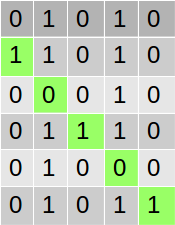
\includegraphics[scale=0.4]{figuras/pmv/notBit.png}}
    \caption{Operador de negação de bit.}
    \label{fig:operadorNegacaoBit}
\end{figure}

Para as vizinhanças da solução foram usados dois tipos de operações, uma sobre $x$ e outra sobre $y$, em $x$ foram usados 4 tipos de operações descritos a seguir, ao passo que para $y$ foram usadas duas operações, o operador de Negação de Bit (coletar um item se não estiver presente ou deixar de coletá-lo caso contrário, exemplificado na Figura~\ref{fig:operadorNegacaoBit}).
Em resumo, a combinação dos movimentos em $x$ e $y$ geram 8 vizinhanças diferentes.
Nessa abordagem, cada solução possui muitos vizinhos, sendo o total calculado pela Equação.~\eqref{eq:neighboorSize}.

\begin{equation} \label{eq:neighboorSize}
    |\Lambda(x, y)| = \frac{4nm(n - 1)}{2} + \frac{4n(n - 1)}{2} = 2n(n - 1)(m + 1) = \Theta(m\;n^2)
\end{equation}

\label{subsec:localSerach:neighborhoods}
As operações na rota $x$ possuem $\frac{n (n -1)}{2}$ vizinhos, a operação de Troca (Swap, Figura~\ref{fig:operadorSwap}) consiste de trocar cada par de inteiros no vetor, outrossim a operação 2-Opt consiste em reverter um grupo de elementos formado por cada par de inteiros do vetor.
A operação de Shift consiste de mover todos os elementos uma posição para a esquerda (Figura~\ref{fig:operadorShiftLeft}) ou direita (Figura~\ref{fig:operadorShiftRight}) dentro de um par de elementos.

\begin{figure}%
    \centering
    \subfloat[Troca]{{
        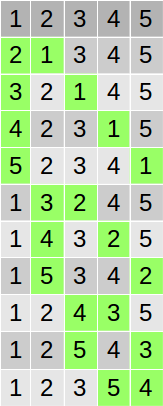
\includegraphics[scale=0.4]{figuras/pmv/swap.png}
        \label{fig:operadorSwap}
    }}%
    \qquad
    \subfloat[Inversão]{{
        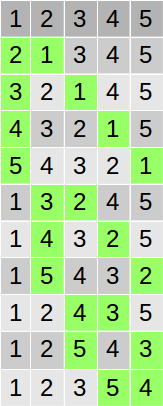
\includegraphics[scale=0.4]{figuras/pmv/inversion.png}
        \label{fig:operadorInversion}
    }}%
    \caption{Vizinhanças troca e inversão}%
    \label{fig:swapInversion}%
\end{figure}

\begin{figure}%
    \centering
    \subfloat[Shift left]{{
        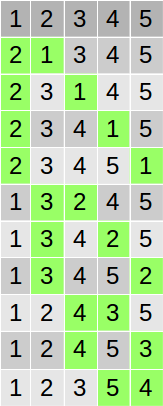
\includegraphics[scale=0.4]{figuras/pmv/shiftLeft.png}
        \label{fig:operadorShiftLeft}
    }}%
    \qquad
    \subfloat[Shift right]{{
        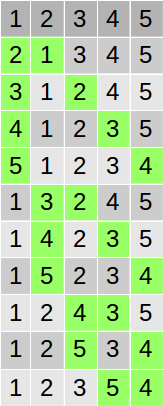
\includegraphics[scale=0.4]{figuras/pmv/shiftRight.png}
        \label{fig:operadorShiftRight}
    }}%
    \caption{Vizinhanças Shift}%
    \label{fig:shiftLeftRight}%
\end{figure}
